\newthought{\textbf{Arya Saputra - 2020903430009 - TRKJ 3B}}

\newday{\textbf{01 Desember 2022}}
\begin{enumerate}
\item Kendala dan Solusi
Pada pertemuan hari ini, kegiatan yang dilakukan adalah menginstall Apache Hadoop. Selama praktikum tidak mengalami kendala.


\item Kesimpulan
Berhasil melakukan instalasi hadoop berikut ini gambar hasil verifikasi instalasi hadoop version 

\begin{figure}[!ht]
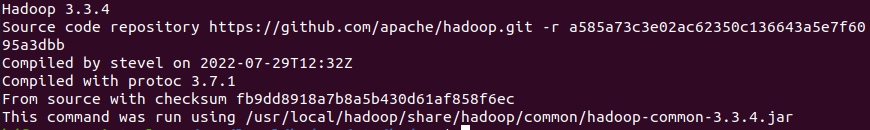
\includegraphics[width=\textwidth]{AryaSyahputra/hadoop version}
\caption{Verifikasi Hasil Instalasi Hadoop}
\label{gam:Hadoop-version}
\end{figure}
\end{enumerate}

\newday{\textbf{02 Desember 2022}}
\begin{enumerate}
\item Kendala
sudah berhasil menginstall hadoop

\item solusi
menginstal ulang ubuntu

\item Kesimpulan
setelah menginstall ulang ubuntu, instalasi dan konfigurasi hadoop berhasil

\begin{figure}[!ht]
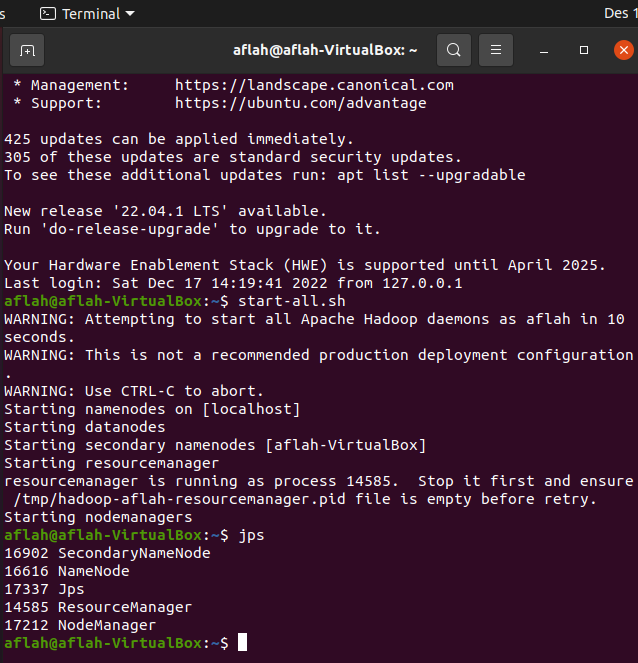
\includegraphics[width=\textwidth]{AryaSyahputra/jps}
\caption{Verifikasi Hasil Instalasi Hadoop}
\label{gam:instalasi-hadoop}
\end{figure}
\begin{figure}[!ht]
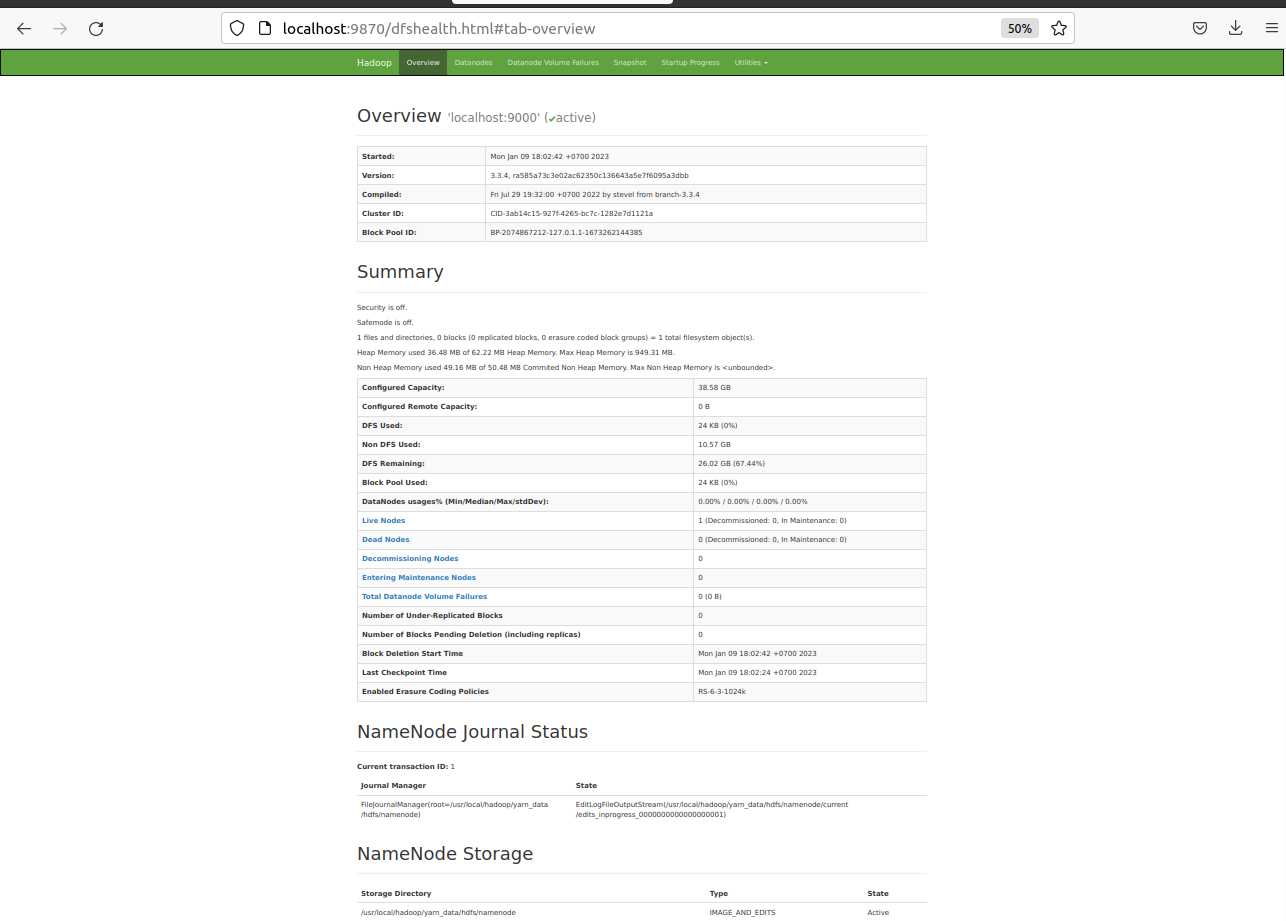
\includegraphics[width=\textwidth]{AryaSyahputra/localhos1}
\caption{Verifikasi Hasil Instalasi Hadoop}
\label{gam:instalasi-hadoop}
\end{figure}
\begin{figure}[!ht]
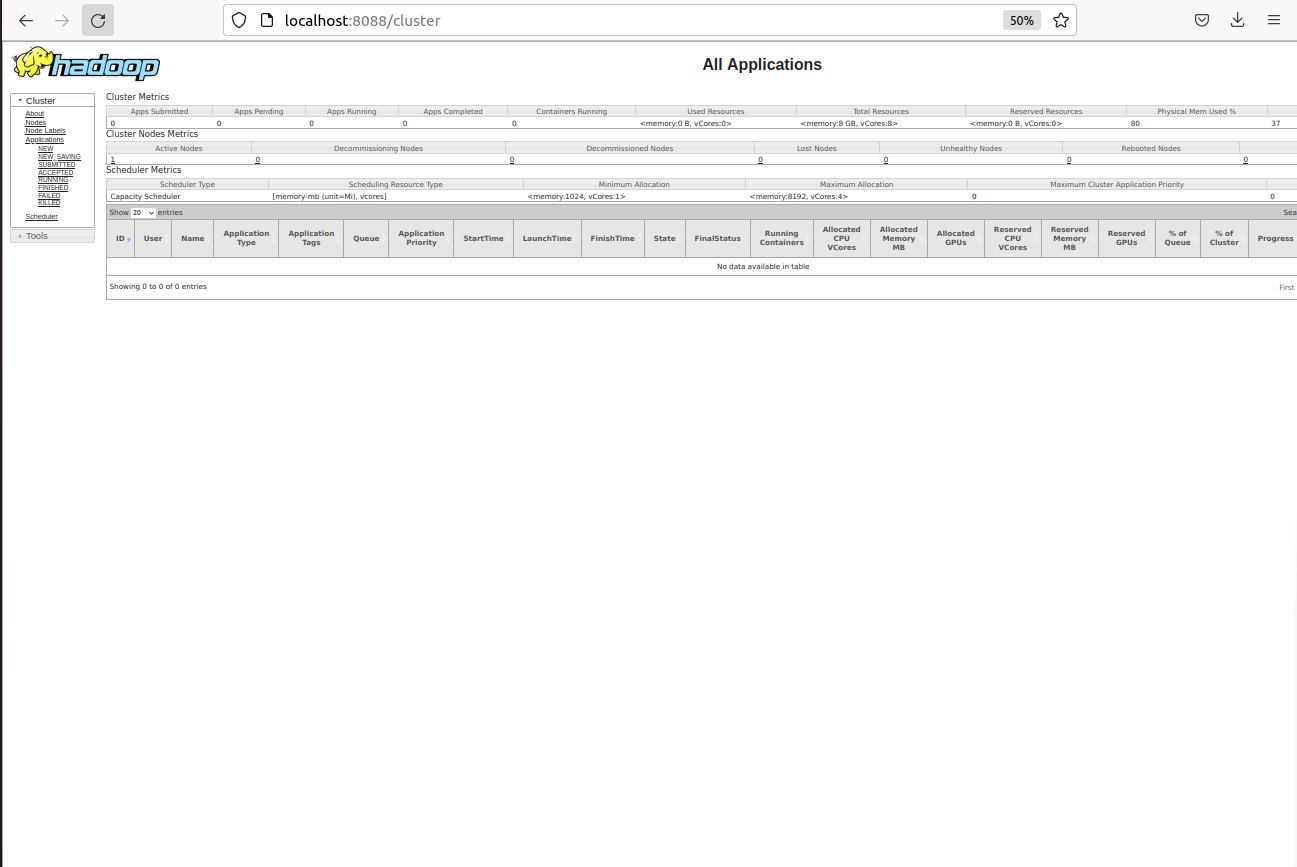
\includegraphics[width=\textwidth]{AryaSyahputra/localhos2}
\caption{Verifikasi Hasil Instalasi Hadoop}
\label{gam:instalasi-hadoop}
\end{figure}
\end{enumerate}

\clearpage
\newday{\textbf{15 Desember 2022}}
\begin{enumerate}
\item Kendala dan Solusi



\item Kesimpulan



\end{enumerate}

